\chapter{Hiện thực hệ thống}
% \section{Công nghệ sử dụng}
% Để hiện thực hệ thống, nhóm quyết định sử dụng các công nghệ sau:
% \begin{itemize}
%     \item ReactJS: Hiện thực UI, frontend.
%     \item Java Springboot: Hiện thực microservice, backend.
%     \item PostgresSQL: Hệ cơ sở dữ liệu lưu trữ thông tin.
%     \item Kubernetes: Deploy các microservice.
%     \item Minikube: Chạy Kubernetes cluster trên local.
%     \item Terraform: Khởi tạo 
% \end{itemize}

% \section{Giới hạn phạm vi}
% \subsection{Về mặt nghiệp vụ}
% \noindent Sau khi bàn bạc, nhóm đi tới thống nhất là sẽ hiện thực phần Trang chủ (Home page - Catalog), vì đó là thành phần mà người dùng sẽ gặp đầu tiên khi bắt đầu truy cập vào hệ thống.
% \subsection{Về mặt thành phần hệ thống}
% \noindent Sau khi cân nhắc kỹ lưỡng, để đảm bảo cho phiên bản demo thể hiện được trọn vẹn và đầy đủ nhất các tính chất cốt lõi của hệ thống, nhóm đã giới hạn phạm vi hiện thực của hệ thống xuống còn các thành phần như sau:
% \begin{itemize}
%     \item Frontend: Trang chủ - Catalog, thể hiện danh sách các mặt hàng đang được bày bán 
%     \item Backend: Catalog service, cung cấp API danh sách sản phẩm.
%     \item Minikube cluster: Cung cấp môi trường Kubernetes cluster local trên máy tính cá nhân.
%     \item Deployment: Thành phần cơ bản nhất của hệ thống, dùng để quản lý trực tiếp các pod.
%     \item Service: Một lớp ảo hóa để các thành phần khác có thể truy cập tới các pod.
%     \item Ingress: Đóng vai trò như reverse proxy, cung cấp API gateway để kết nối từ bên ngoài cluster tới service.
%     \item Horizontal Pod Autoscaler: Dùng để tăng hoặc giảm số pod một cách tự động, dựa trên các thông số (metrics) của chính các pod đó.
% \end{itemize}
\section{Lựa chọn công nghệ và thư viện}
\subsection{Frontend}
\noindent Để hiện thực giao diện người dùng, nhóm đã lựa chọn ReactJS, một thư viện JavaScript phổ biến được phát triển bởi Facebook. ReactJS giúp xây dựng giao diện người dùng một cách dễ dàng, linh hoạt và hiệu quả. Nó sử dụng cơ chế Virtual DOM để tối ưu hóa hiệu suất, giúp người dùng có trải nghiệm tốt hơn.\\[0.5cm]
Cùng với ReactJS, nhóm cũng sử dụng thêm các library/framework/tool để hỗ trợ như:
\begin{itemize}
    \item \textbf{React Router}: Là một thư viện mã nguồn mở để quản lý điều hướng (routing) trong các ứng dụng
    web. Thay vì tải lại toàn bộ trang web khi người dùng thực hiện các thao tác điều hướng, React
    Router cho phép ứng dụng thay đổi nội dung trên cùng một trang một cách nhanh chóng và mượt
    mà, giúp tăng trải nghiệm người dùng.
    \item \textbf{Redux}: Redux là một thư viện quản lý trạng thái (state management) cho ứng dụng JavaScript, thường được sử dụng trong các ứng dụng React. Nó giúp quản lý trạng thái của ứng dụng một cách hiệu quả và dễ dàng theo dõi.
    \item \textbf{Reduc Toolkit}: Redux Toolkit là một bộ công cụ (toolkit) được thiết kế để giảm bớt sự phức tạp khi sử dụng Redux và cung cấp các tiện ích hữu ích để viết code một cách nhanh chóng và hiệu quả hơn. 
    \item \textbf{React Persist}: Redux Persist là một thư viện cho phép lưu trữ trạng thái của ứng dụng Redux vào bộ nhớ cục bộ của trình duyệt, giúp duy trì trạng thái khi người dùng tải lại trang hoặc đóng/mở trình duyệt.
    \item \textbf{Axios}: Là một thư viện HTTP client dựa trên Promise dùng để thực hiện các yêu cầu HTTP từ trình duyệt và Node.js. Axios giúp đơn giản hóa việc giao tiếp với server, hỗ trợ các phương thức HTTP như GET, POST, PUT, DELETE và xử lý dữ liệu trả về dễ dàng.
    \item \textbf{Thư viện Antd}: Là một thư viện UI component dành cho React, cung cấp một loạt các thành phần giao diện người dùng phong phú và đa dạng theo phong cách Ant Design. Thư viện này giúp tăng tốc quá trình phát triển giao diện người dùng với thiết kế nhất quán và đẹp mắt.
    \item \textbf{Styled-components}: Là một thư viện cho phép viết CSS trực tiếp trong JavaScript bằng cách sử dụng tagged template literals. Styled-components giúp tạo các component với styles riêng biệt, dễ duy trì và tái sử dụng, đồng thời hỗ trợ tính năng theming và tạo CSS động.
    \item \textbf{SASS}: Là một tiền xử lý CSS giúp viết mã CSS dễ dàng hơn và mạnh mẽ hơn bằng cách cung cấp các tính năng như biến, lồng ghép (nesting), mixin, và thừa kế (inheritance). SASS giúp viết mã CSS có cấu trúc rõ ràng và dễ duy trì hơn.
    \item \textbf{Vite}: Là một công cụ build và phát triển nhanh chóng dành cho các dự án web hiện đại, đặc biệt là các ứng dụng sử dụng JavaScript và TypeScript. Vite cung cấp khả năng hot module replacement (HMR), giúp phát triển nhanh hơn và tối ưu hóa thời gian build sản phẩm cuối cùng.
    \item \textbf{Nginx}:Là một máy chủ web (web server) mạnh mẽ, thường được sử dụng làm reverse proxy, load balancer, mail proxy, và HTTP cache. Nginx nổi tiếng với hiệu suất cao, khả năng xử lý lượng truy cập lớn, và dễ cấu hình.
    \item \textbf{Formik}: Là một thư viện quản lý form cho React, giúp quản lý trạng thái của form, xác thực dữ liệu, và xử lý sự kiện một cách dễ dàng và hiệu quả.
    \item \textbf{Yup}: Là một thư viện xác thực dữ liệu (data validation) cho JavaScript và TypeScript, giúp xác thực dữ liệu đầu vào từ người dùng một cách dễ dàng và linh hoạt.
\end{itemize}
\noindent Ngoài ra, ReactJS còn hỗ trợ một loạt các packages khác như react-query, react-hook-form, react-toastify, react-icons, react-select, react-table, react-datepicker, react-dropzone, react-quill, react-router-dom, react-slick, react-spring, react-transition-group, react-use, react-window, react-virtualized, react-youtube, v.v. giúp tăng cường khả năng phát triển và tối ưu hóa hiệu suất của ứng dụng.
\subsection{Backend}
\subsubsection{Java Spring Boot}
\noindent Để hiện thực các microservice, nhóm đã lựa chọn Java Spring Boot, một framework phổ biến được sử dụng để xây dựng các ứng dụng Java nhanh chóng và hiệu quả. Spring Boot giúp giảm thiểu thời gian và công sức cần thiết để xây dựng ứng dụng Java, đồng thời cung cấp các tính năng như dependency injection, auto-configuration, và embedded server, giúp tăng tốc quá trình phát triển và triển khai ứng dụng.

\subsubsection{Golang Fiber}
\noindent Golang (Go) là một ngôn ngữ lập trình mã nguồn mở được phát triển bởi Google, được thiết kế để đơn giản, hiệu quả và dễ sử dụng. Nó có cú pháp rõ ràng, hiệu suất cao, hỗ trợ quản lý đồng thời và garbage collection tự động. Go hỗ trợ đa nền tảng và có một hệ sinh thái phong phú với thư viện tiêu chuẩn và cộng đồng phát triển mạnh mẽ.\\[0.5cm]

\noindent Fiber là một framework web được viết bằng ngôn ngữ lập trình Go (Golang), lấy cảm hứng từ ExpressJS của NodeJS, với mục tiêu cung cấp một framework nhẹ, nhanh và thân thiện với lập trình viên.
\subsubsection{NodeJS kết hợp ExpressJS} 
\noindent Node.js là một nền tảng phát triển ứng dụng web mã nguồn mở, được xây dựng trên JavaScript Engine của Chrome (V8 Engine). Node.js cho phép viết mã JavaScript ở phía server, giúp xây dựng các ứng dụng web hiệu quả và mạnh mẽ. \\[0.5cm]
\noindent Express là một framework web cho Node.js, giúp xây dựng các ứng dụng web và API một cách nhanh chóng và dễ dàng.
\subsubsection{SocketIO}
\noindent Socket.IO là một thư viện JavaScript cho phép thiết lập kết nối real-time giữa client và server thông qua WebSockets hoặc các kỹ thuật khác như polling hay long-polling. Socket.IO giúp xây dựng các ứng dụng real-time như chat, game, hoặc các ứng dụng cần cập nhật dữ liệu một cách nhanh chóng và liên tục.

\subsection{Database}
\noindent Để lưu trữ dữ liệu, nhóm đã sử dụng PostgreSQL, một hệ quản trị cơ sở dữ liệu mã nguồn mở phổ biến, mạnh mẽ và linh hoạt. PostgreSQL hỗ trợ nhiều tính năng như ACID, MVCC, JSON, và hỗ trợ các kiểu dữ liệu phong phú, giúp lưu trữ và truy vấn dữ liệu một cách hiệu quả.

\subsection{Message Broker}
\noindent RabbitMQ là một hệ thống message broker mã nguồn mở, được sử dụng để truyền thông tin giữa các ứng dụng khác nhau. RabbitMQ hỗ trợ nhiều giao thức như AMQP, MQTT, STOMP, và HTTP, giúp kết nối các ứng dụng với nhau một cách linh hoạt và hiệu quả.

\subsection{Triển khai}
\noindent Để triển khai hệ thống, nhóm đã sử dụng Kubernetes, một hệ thống mã nguồn mở giúp quản lý và triển khai các containerized applications. Kubernetes cung cấp các tính năng như auto-scaling, self-healing, và load balancing, giúp tăng cường hiệu suất và tin cậy của hệ thống.
\subsubsection{Docker}
\noindent Docker là một nền tảng mã nguồn mở giúp xây dựng, vận chuyển và chạy các ứng dụng trong các container. Docker giúp tạo ra môi trường đồng nhất giữa các môi trường phát triển, thử nghiệm và triển khai, giúp tăng tốc quá trình phát triển và triển khai ứng dụng.
\subsubsection{Kubernetes}
Kubernetes là một hệ thống mã nguồn mở để tự động hóa việc triển khai, mở rộng và quản lý các ứng dụng container. Nó giúp điều phối các container trên một cụm (cluster) máy chủ, đảm bảo khả năng mở rộng, tự phục hồi và dễ dàng quản lý. Kubernetes cung cấp các tính năng như cân bằng tải, tự động phát hiện dịch vụ, quản lý cấu hình và bí mật, và tự động mở rộng ứng dụng dựa trên tải công việc.
\subsubsection{Minikube}
Minikube là một công cụ giúp chạy Kubernetes cục bộ trên máy tính cá nhân. 
Nó tạo ra một cụm Kubernetes một nút (single-node cluster) để phát triển và thử nghiệm, cho phép bạn trải nghiệm và học tập Kubernetes mà không cần hạ tầng phức tạp. 
Minikube hỗ trợ nhiều nền tảng như Linux, macOS và Windows, và cung cấp đầy đủ các tính năng của Kubernetes trong một môi trường dễ cài đặt và sử dụng.
\subsubsection{Keda}
Keda (Kubernetes-based Event-Driven Autoscaling) là một công cụ mã nguồn mở giúp tự động mở rộng các ứng dụng dựa trên sự kiện trong Kubernetes. 
Keda giúp mở rộng các ứng dụng dựa trên các nguồn sự kiện như hàng đợi, chủ đề, hoặc bất kỳ nguồn sự kiện nào khác, 
giúp tối ưu hóa việc sử dụng tài nguyên và giảm chi phí vận hành.
\subsubsection{Prometheus}
Prometheus là một hệ thống giám sát mã nguồn mở được sử dụng để giám sát và cảnh báo cho các ứng dụng và 
hệ thống phân tán. Nó sử dụng kiến trúc server-client đơn giản, ngôn ngữ truy vấn PromQL để phân tích dữ liệu, 
và hỗ trợ giám sát đa chiều với khả năng áp dụng nhãn cho metrics. Prometheus cũng cung cấp tính năng cảnh báo tích hợp và có khả năng mở rộng linh hoạt.
\subsection{Kiểm thử}
K6 là một công cụ mã nguồn mở mạnh mẽ được sử dụng để kiểm thử hiệu suất và tải của ứng dụng. Với khả năng tạo và thực thi các kịch bản kiểm thử linh hoạt, K6 cho phép bạn mô phỏng hàng trăm hoặc thậm chí hàng ngàn người dùng truy cập cùng một lúc vào ứng dụng của bạn để đo lường thời gian phản hồi, tải trọng máy chủ và các chỉ số hiệu suất khác.
\section{Mã nguồn}
\subsection{Quản lý mã nguồn}
\noindent Git là một hệ thống quản lý phiên bản mã nguồn mở rất phổ biến, được sử dụng để quản lý mã nguồn trong các dự án phần mềm. Nó được Linus Torvalds phát triển vào năm 2005 và đã trở thành một công cụ không thể thiếu trong cộng đồng phần mềm mã nguồn mở. Git giúp các nhà phát triển dễ dàng và hiệu quả làm việc trên các phiên bản khác nhau của cùng một dự án, từ đó hỗ trợ quản lý và giám sát quá trình phát triển phần mềm. \\[0.5cm]
Nhóm đã lựa chọn \textbf{GitHub} để quản lý mã nguồn. GitHub là một dịch vụ lưu trữ mã nguồn trực tuyến (source code repository) và nền tảng hợp tác phát triển phần mềm dựa trên Git. GitHub cho phép các nhà phát triển lưu trữ, quản lý và chia sẻ mã nguồn của các dự án phần mềm.\\[0.5cm]
Ngoài ra, để việc đóng góp của các thành viên được diễn ra một cách bài bản và khoa học, nhóm đã định ra một bộ quy tắc về cách đặt tên branch, cách tạo, duyệt, gộp nội dung từ pull request vào branch chính, sẽ được trình bày cụ thể hơn ở phần phụ lục.

\subsection{Cấu trúc mã nguồn}
\noindent Nhóm đã tận dụng Github để quản lý mã nguồn cho 2 nội dung quan trọng nhất của đồ án, là báo cáo (được viết bằng Latex) và hệ thống, tương ứng với 2 repository. Mỗi repository đều có README ghi chú đầy đủ các nội dung hướng dẫn, giúp mỗi thành viên có thể nắm được các thông tin cơ bản của repository, đồng thời thực hiện các bước thiết lập nếu cần, trước khi có thể đóng góp nội dung vào đó.
\subsubsection{Mã nguồn báo cáo}
\noindent Do nội dung báo cáo không ít, vì vậy nhóm không ghi hết toàn bộ nội dung vào 1 file tex duy nhất, mà được chia ra thành nhiều file với cấu trúc như hình \ref{fig:thesis_source_code_structure}:
\begin{itemize}
    \item Thư mục \textbf{images}: Chứa toàn bộ các hình ảnh được sử dụng cho báo cáo. Bên trong còn được chia ra thành nhiều thư mục con, ứng với từng thành viên. Mỗi thành viên sẽ tự quản lý những hỉnh ảnh mà mình sử dụng trong báo cáo.
    \item Thư mục \textbf{sections}: Chứa nội dung của các chương trong báo cáo. Mỗi chương sẽ là 1 file tex riêng.
    \item File \textbf{main.tex}: Là khung xương của toàn bộ báo cáo, chứa các thiết lập, đồng thời là điểm bắt đầu để latex có thể biên tập nội dung.
    \item File \textbf{README.md}: Chứa đựng các thông tin cần thiết về repository. 
\end{itemize}
\begin{figure}[H]
    \begin{center}
        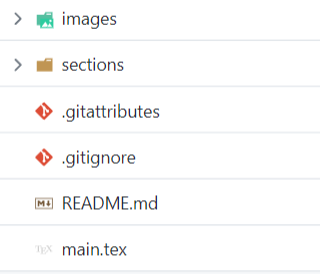
\includegraphics[scale = 1.5]{images/hanh/thesis-source-code-screenshot.png}
        \vspace*{2mm}
    \end{center}
    \caption{Cấu trúc mã nguồn của báo cáo}
    \label{fig:thesis_source_code_structure}

\end{figure}
\subsubsection{Mã nguồn hệ thống}
\noindent Nhằm đáp ứng cho yêu cầu của đề tài và giải pháp tương ứng, hệ thống được triển khai theo kiến trúc microservice, với mỗi microservice sẽ đáp ứng một chức năng cụ thể. Để việc quản lý mã nguồn các dịch vụ này diễn ra một cách tập trung và đồng bộ, toàn bộ mã nguồn hệ thống sẽ được lưu trữ trong một repository duy nhất, được triển khai theo kiến trúc monorepo, bằng cách sử dụng \textbf{yarn workspace} và \textbf{turbo}. Cấu trúc cây thư mục sẽ trông như hình \ref{fig:ecomm_app_source_code}.
\begin{itemize}
    \item Thư mục \textbf{apps}: Chứa toàn bộ mã nguồn của các microservice. Các dịch vụ này được chia vào 3 thư mục con:
    \begin{itemize}
        \item \textbf{backend}: Chứa các microservice với mục đích hiện thực các logic hệ thống, đồng thời chứa các API để trình duyệt có thể giao tiếp.
        \item \textbf{database}: Chứa các microservice với mục đích truy xuất database. Các logic khi query, insert với database sẽ được thực hiện bởi các dịch vụ này.
        \item \textbf{frontend}: Chứa mã nguồn cho các microservice dùng để hiển thị giao diện cho người dùng. Hiện tại, do không đủ thời gian nên nhóm vẫn chưa thực hiện kiến trúc microservice cho frontend.
    \end{itemize}
    \item Thư mục \textbf{deploy}: Chứa các cấu hình phục vụ cho việc triển khai hệ thống. Hiện tại có 2 thư mục con:
    \begin{itemize}
        \item \textbf{k8s-ms}: Chứa các cấu hình phục vụ cho việc triển khai hệ thống thương mại điện tử lên Kubernetes, bao gồm các dịch vụ như ingress, deployment, statefulset, v.v.
        \item \textbf{rabbitmq}: Chứa các cấu hình phục vụ cho việc triển khai RabbitMQ.
    \end{itemize}
\end{itemize}
\begin{figure}[H]
    \begin{center}
        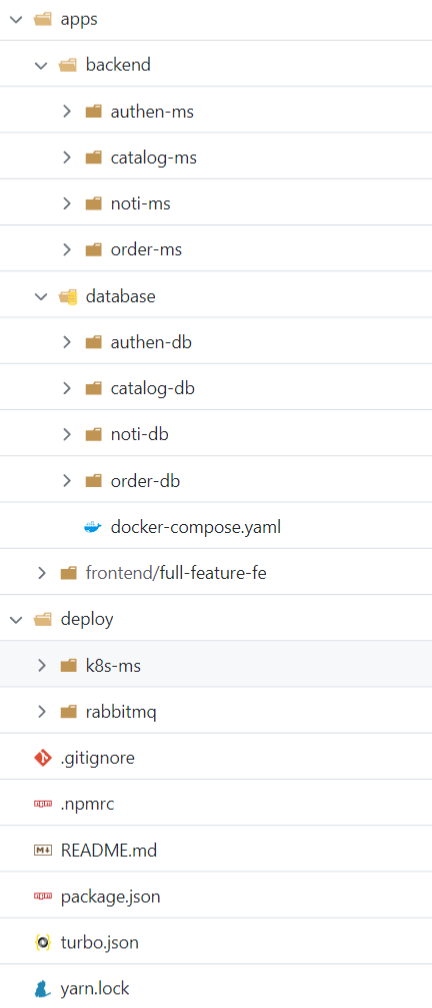
\includegraphics[scale = 1.5]{images/hanh/ecomm-app-source-code.png}
        \vspace*{2mm}
    \end{center}
    \caption{Cấu trúc mã nguồn của hệ thống}
    \label{fig:ecomm_app_source_code}
\end{figure}
\section{Giao diện hệ thống}
\subsection{Trang đăng nhập}
\noindent Sau khi đăng nhập thành công, hệ thống chuyển đến trang chủ, nếu người dùng chưa đăng ký tài khoản, chọn nút đăng ký, hệ thống sẽ chuyển đến trang đăng ký
\begin{figure}[H]
    \begin{center}
    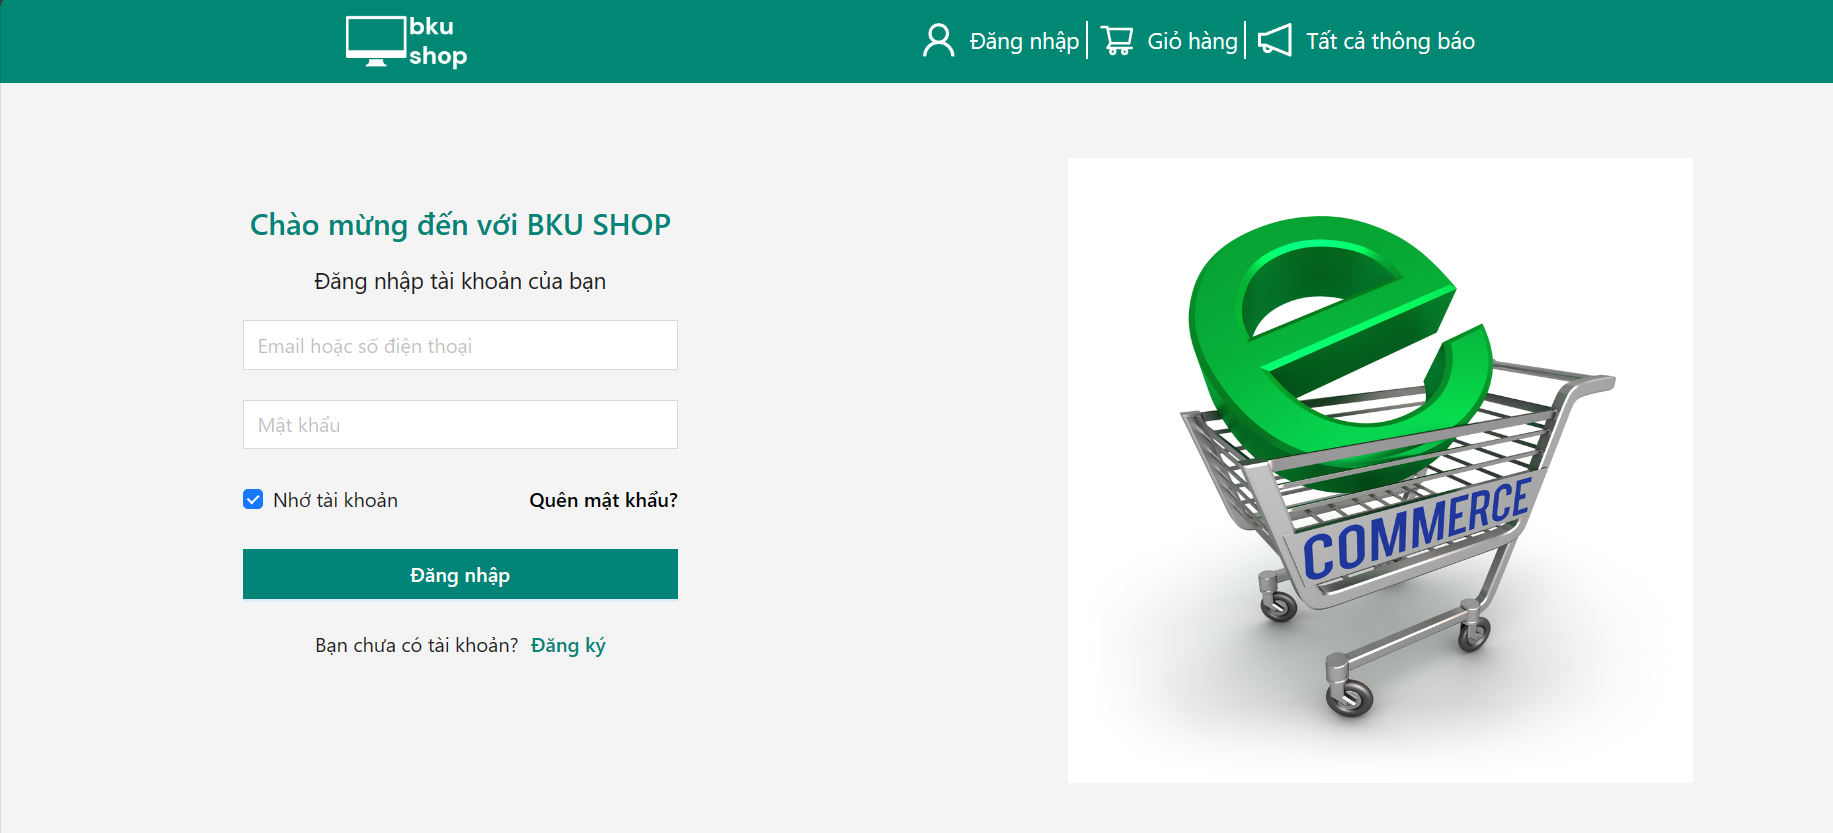
\includegraphics[scale=0.35]{images/hieu/chap-5/login.png}
    \vspace*{3mm}
    \caption{Giao diện trang đăng nhập}
    \end{center}
\end{figure}

\subsection{Trang đăng ký tài khoản}
\noindent Sau khi đăng ký tài khoản thành công, hệ thống chuyển đến trang đăng nhập, nếu đã có tài khoản, chọn nút đăng nhập.
\begin{figure}[H]
    \begin{center}
    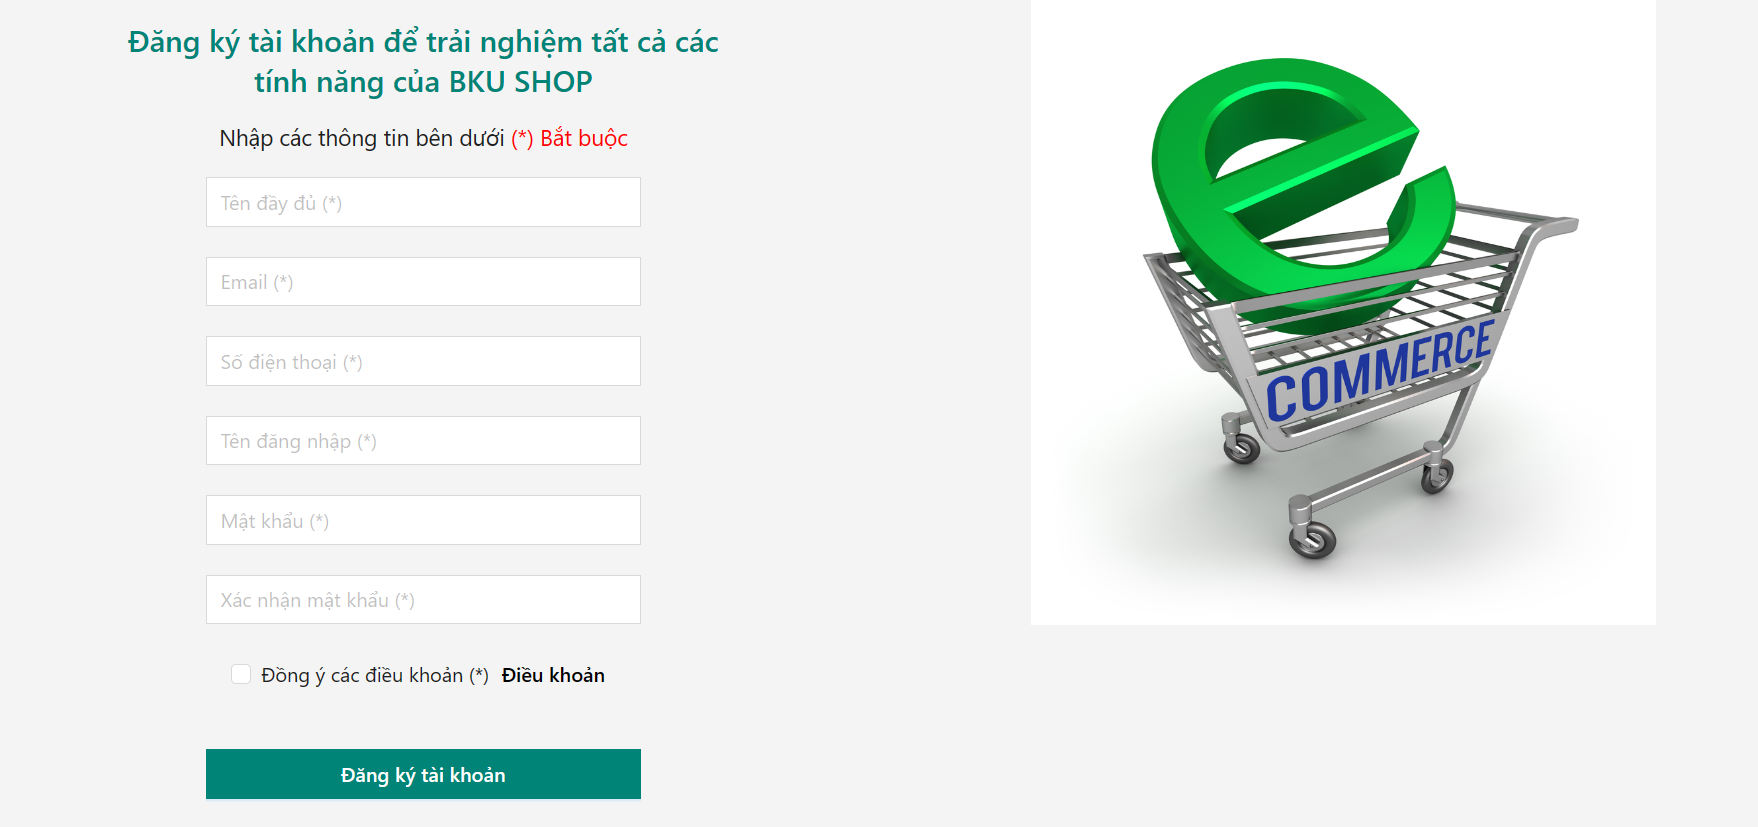
\includegraphics[scale=0.35]{images/hieu/chap-5/signup.png}
    \vspace*{3mm}
    \caption{Giao diện trang đăng ký}
    \end{center}
\end{figure}
\subsection{Trang chủ - Catalog}
\noindent Giao diện trang chủ gồm các thành phần:
\begin{itemize}
    \item Header: Hiển thị logo, tên cửa hàng, nút đăng nhập, giỏ hàng, nút xem thông báo.
    \item Sidebar: Hiển thị danh mục các sản phẩm
    \item Danh sách giảm giá nổi bật
    \item Danh sách tất cả sản phẩm dưới dạng phân trang, thông tin sản phẩm như tên, số lượng trong kho, giá, đánh giá.
    \item Thanh tìm kiếm sản phẩm
    \item Lọc sản phẩm theo khoảng giá
    \item Footer: Hiển thị thông tin liên hệ, thông tin cửa hàng.
    \item Modal: Hiển thị thông tin chi tiết sản phẩm khi người dùng click vào sản phẩm.
\end{itemize}
\begin{figure}[H]
    \begin{center}
    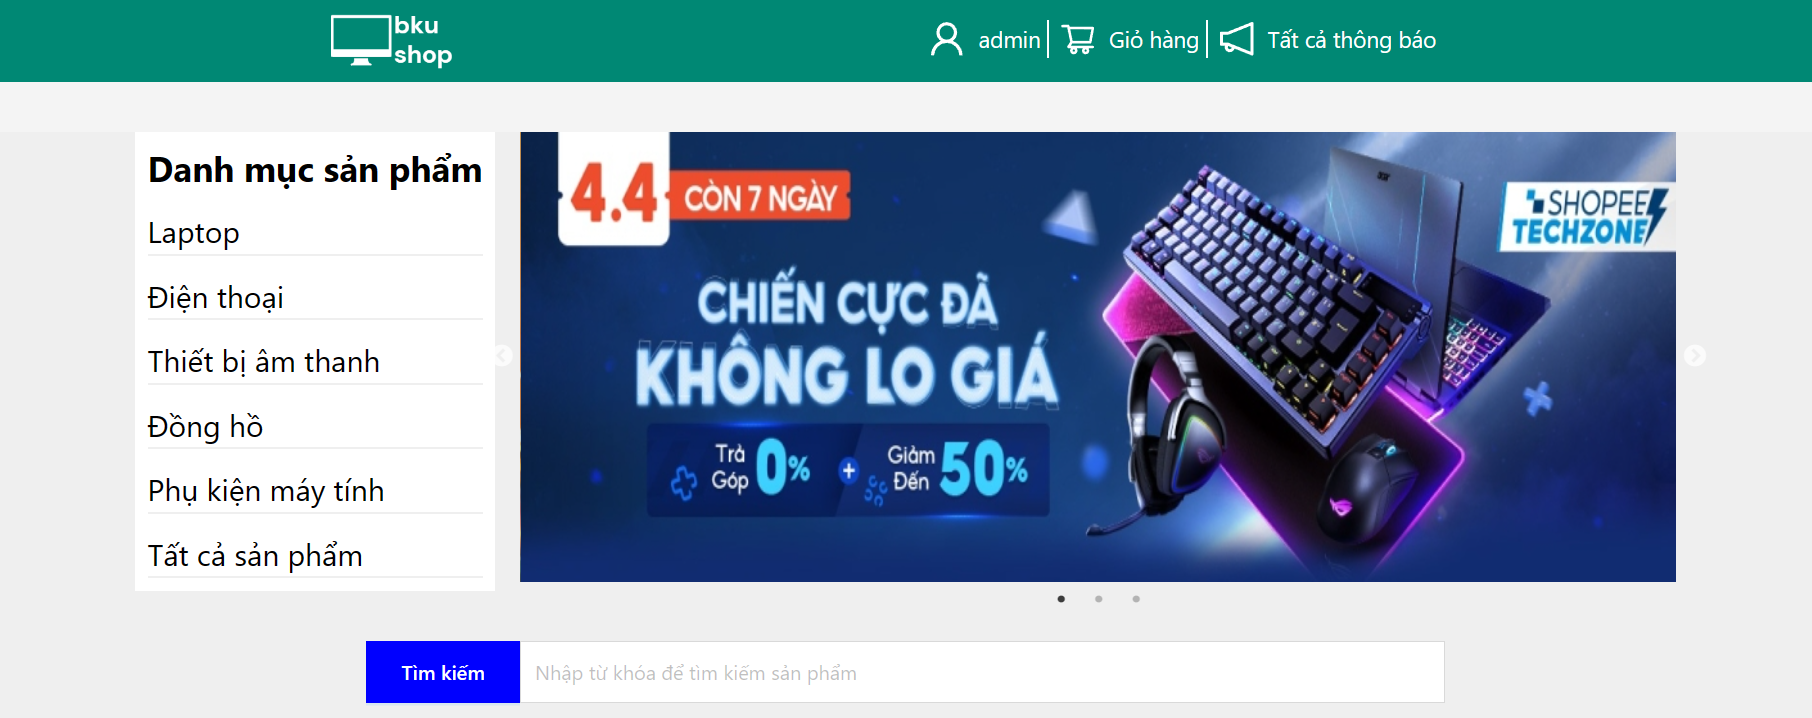
\includegraphics[scale=0.35]{images/hieu/chap-5/catalog-1.png}
    \vspace*{3mm}
    \caption{Giao diện trang chủ - Slider giảm giá - Danh mục sản phẩm}
    \end{center}
\end{figure}

\begin{figure}[H]
    \begin{center}
    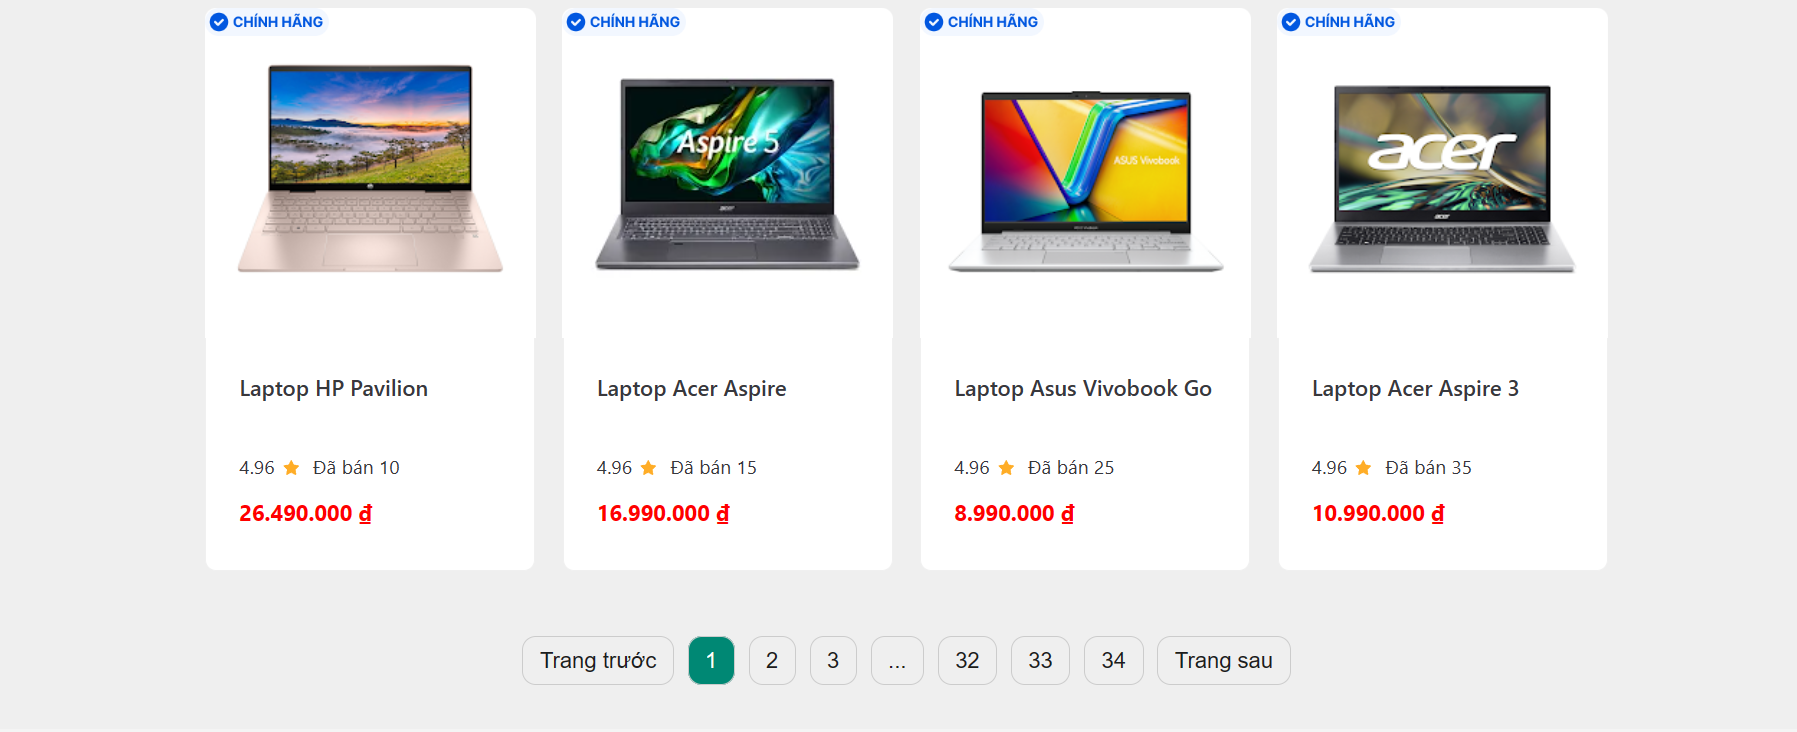
\includegraphics[scale=0.35]{images/hieu/chap-5/catalog-2.png}
    \vspace*{3mm}
    \caption{Giao diện trang chủ - Danh sách sản phẩm }
    \end{center}
\end{figure}

\begin{figure}[H]
    \begin{center}
    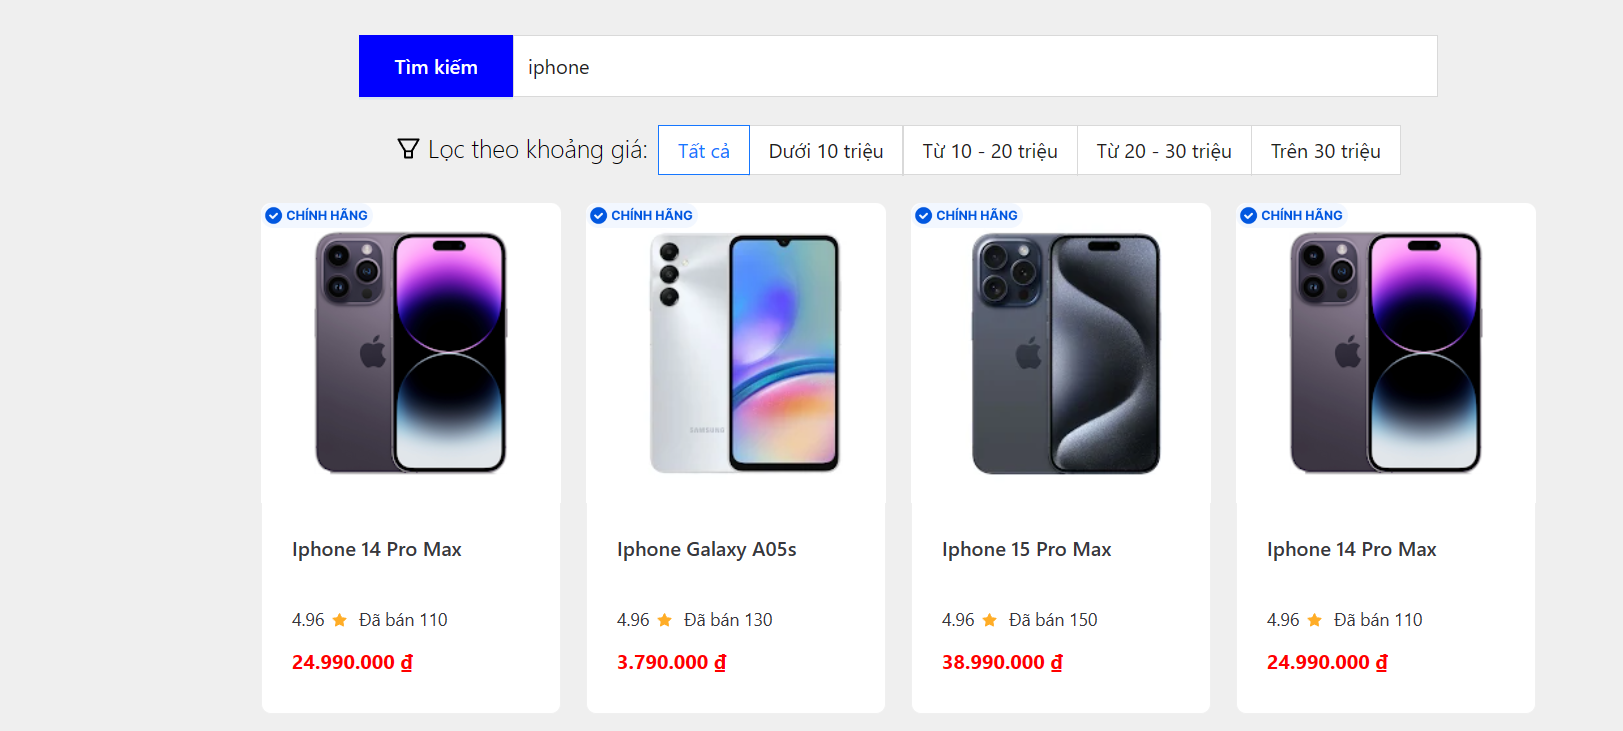
\includegraphics[scale=0.4]{images/hieu/chap-5/search.png}
    \vspace*{3mm}
    \caption{Giao diện trang chủ - Tìm kiếm và lọc sản phẩm }
    \end{center}
\end{figure}
\subsection{Trang chi tiết sản phẩm}
\begin{itemize}
    \item Hiển thị đầy đủ và chi tiết các thông tin từng sản phẩm của cửa hàng.
    \item Chọn nút mua ngay để mua trực tiếp sản phẩm.
    \item Chọn nút thêm vào giỏ hàng để thêm sản phẩm vào giỏ hàng.
\end{itemize}
\begin{figure}[H]
    \begin{center}
    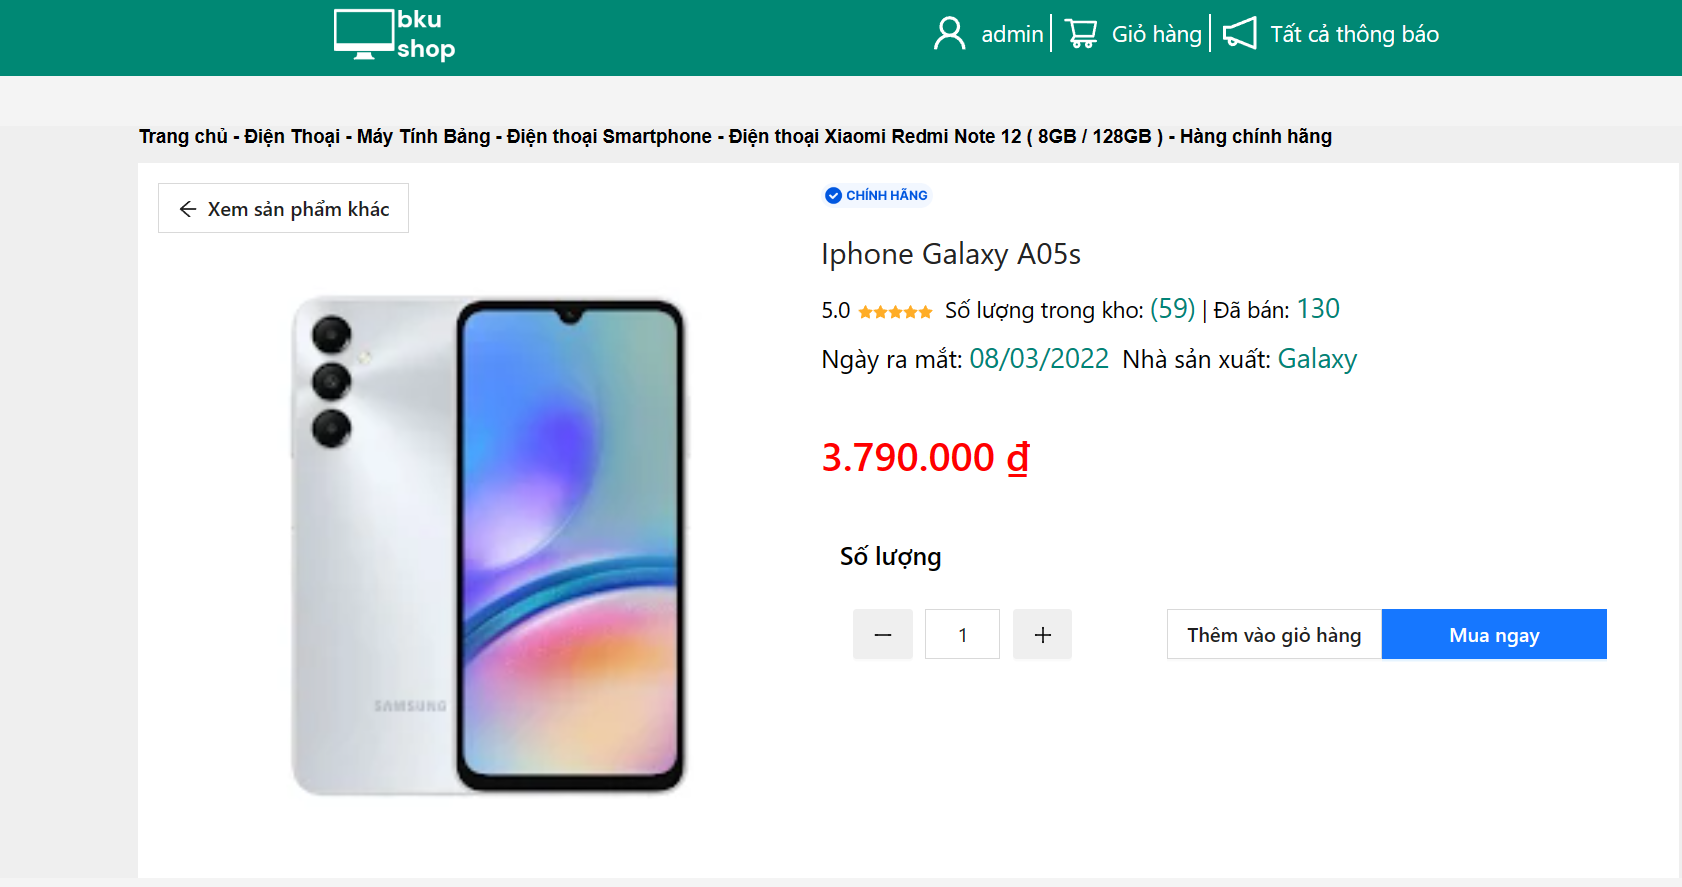
\includegraphics[scale=0.4]{images/hieu/chap-5/product-detail.png}
    \vspace*{3mm}
    \caption{Giao diện trang chi tiết sản phẩm}
    \end{center}
\end{figure}
\subsection{Trang giỏ hàng}
\begin{itemize}
    \item Hiển thị danh sách các sản phẩm người dùng có dự định mua.
    \item Hiển thị số lượng từng sản phẩm, tổng phụ, phí vận chuyển, tổng cuối cùng.
    \item Người dùng có thể điều chỉnh số lượng cũng như xóa sản phẩm khỏi giỏ hàng.
    \item Chọn nút thanh toán để tạo đơn hàng các sản phẩm trong giỏ hàng.
\end{itemize}

\begin{figure}[H]
    \begin{center}
    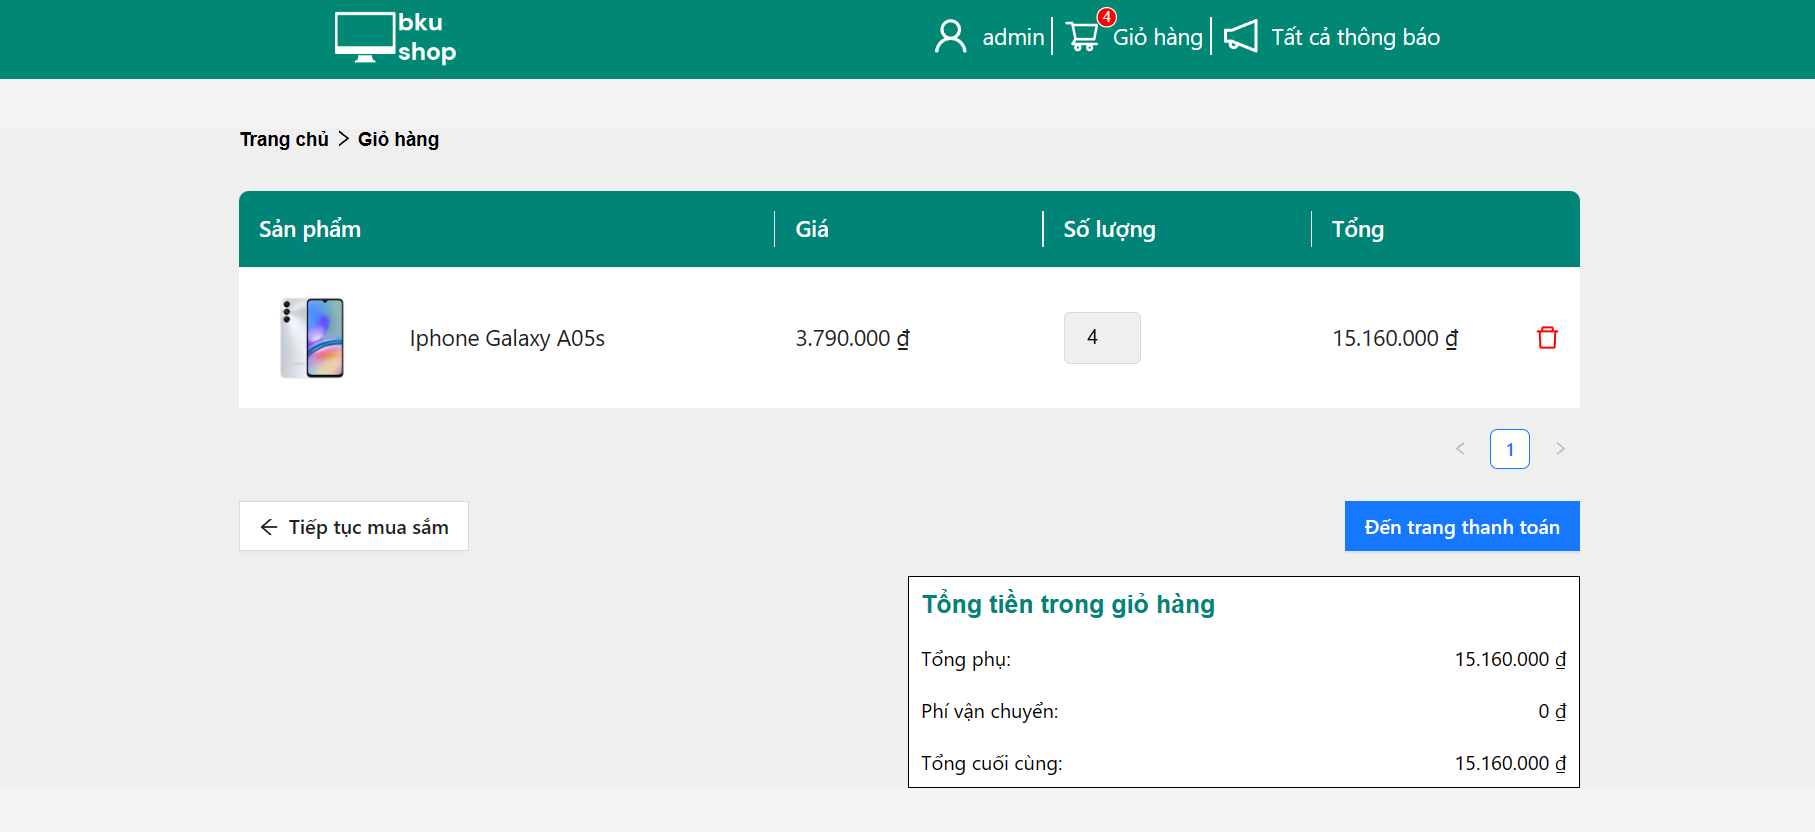
\includegraphics[scale=0.4]{images/hieu/chap-5/cart.png}
    \vspace*{3mm}
    \caption{Giao diện trang giỏ hàng}
    \end{center}
\end{figure}
\subsection{Trang đặt hàng - Thanh toán}
\begin{itemize}
    \item Hiển thị danh sách các sản phẩm người dùng muốn mua.
    \item Hiển thị số lượng từng sản phẩm, tổng phụ, phí vận chuyển, tổng cuối cùng.
    \item Thông tin người dùng, địa chỉ giao hàng.
    \item Chọn nút thanh toán để hoàn tất tạo đơn hàng.
\end{itemize}

\begin{figure}[H]
    \begin{center}
    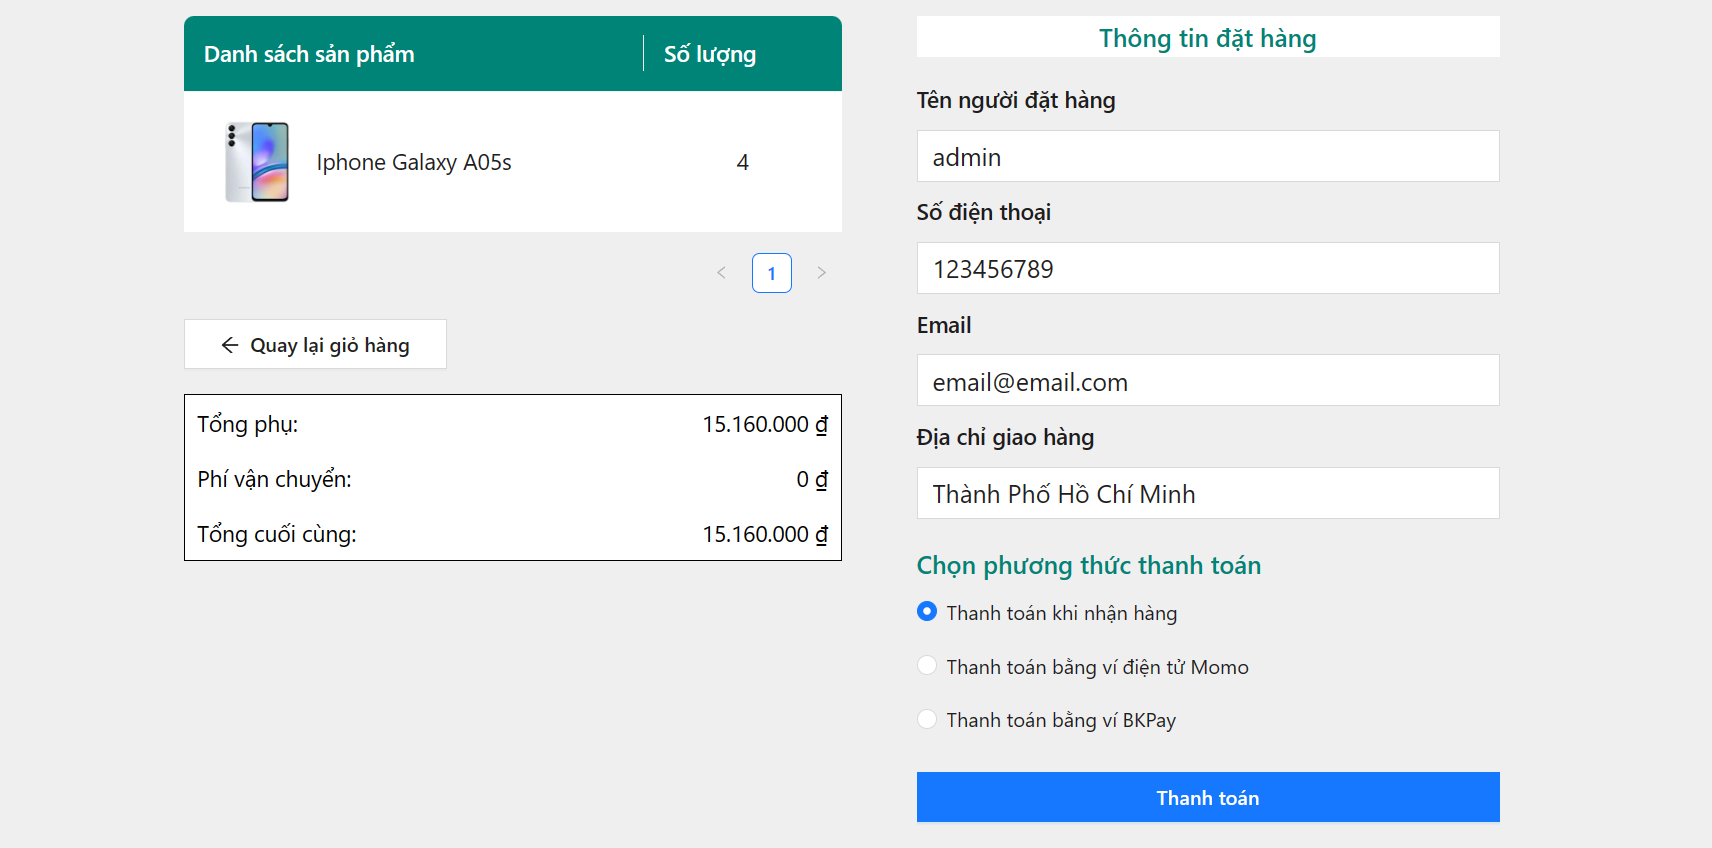
\includegraphics[scale=0.4]{images/hieu/chap-5/payment.png}
    \vspace*{3mm}
    \caption{Giao diện trang đặt hàng}
    \end{center}
\end{figure}
\subsection{Trang quản lý đơn hàng}
\begin{itemize}
    \item Hiển thị danh sách các đơn hàng mà người dùng đã đặt dưới dạng phân trang.
    \item Thông tin đơn hàng như: mã đơn hàng, ngày đặt hàng, tổng tiền, phương thức thanh toán, trạng thái đơn hàng.
    \item Nhấn chọn từng đơn hàng để xem chi tiết hơn.
    \item Lọc đơn hàng theo trạng thái hoặc theo ngày đặt hàng.
\end{itemize}

\begin{figure}[H]
    \begin{center}
    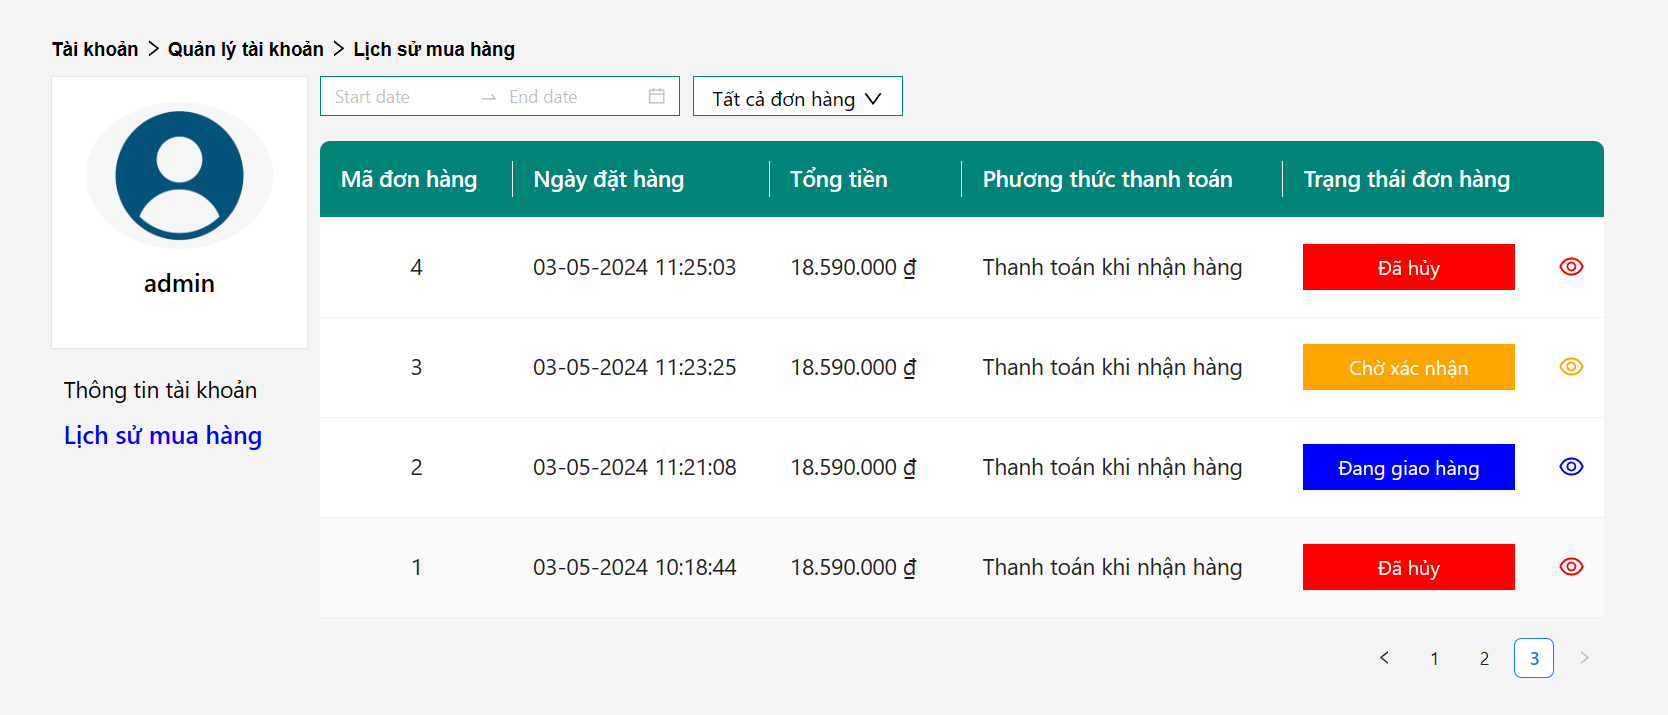
\includegraphics[scale=0.43]{images/hieu/chap-5/ordered.png}
    \vspace*{3mm}
    \caption{Giao diện trang quản lý đơn hàng}
    \end{center}
\end{figure}
\subsection{Trang chi tiết đơn hàng}
\noindent Hiển thị thông tin chi tiết của từng đơn hàng.
\begin{figure}[H]
    \begin{center}
    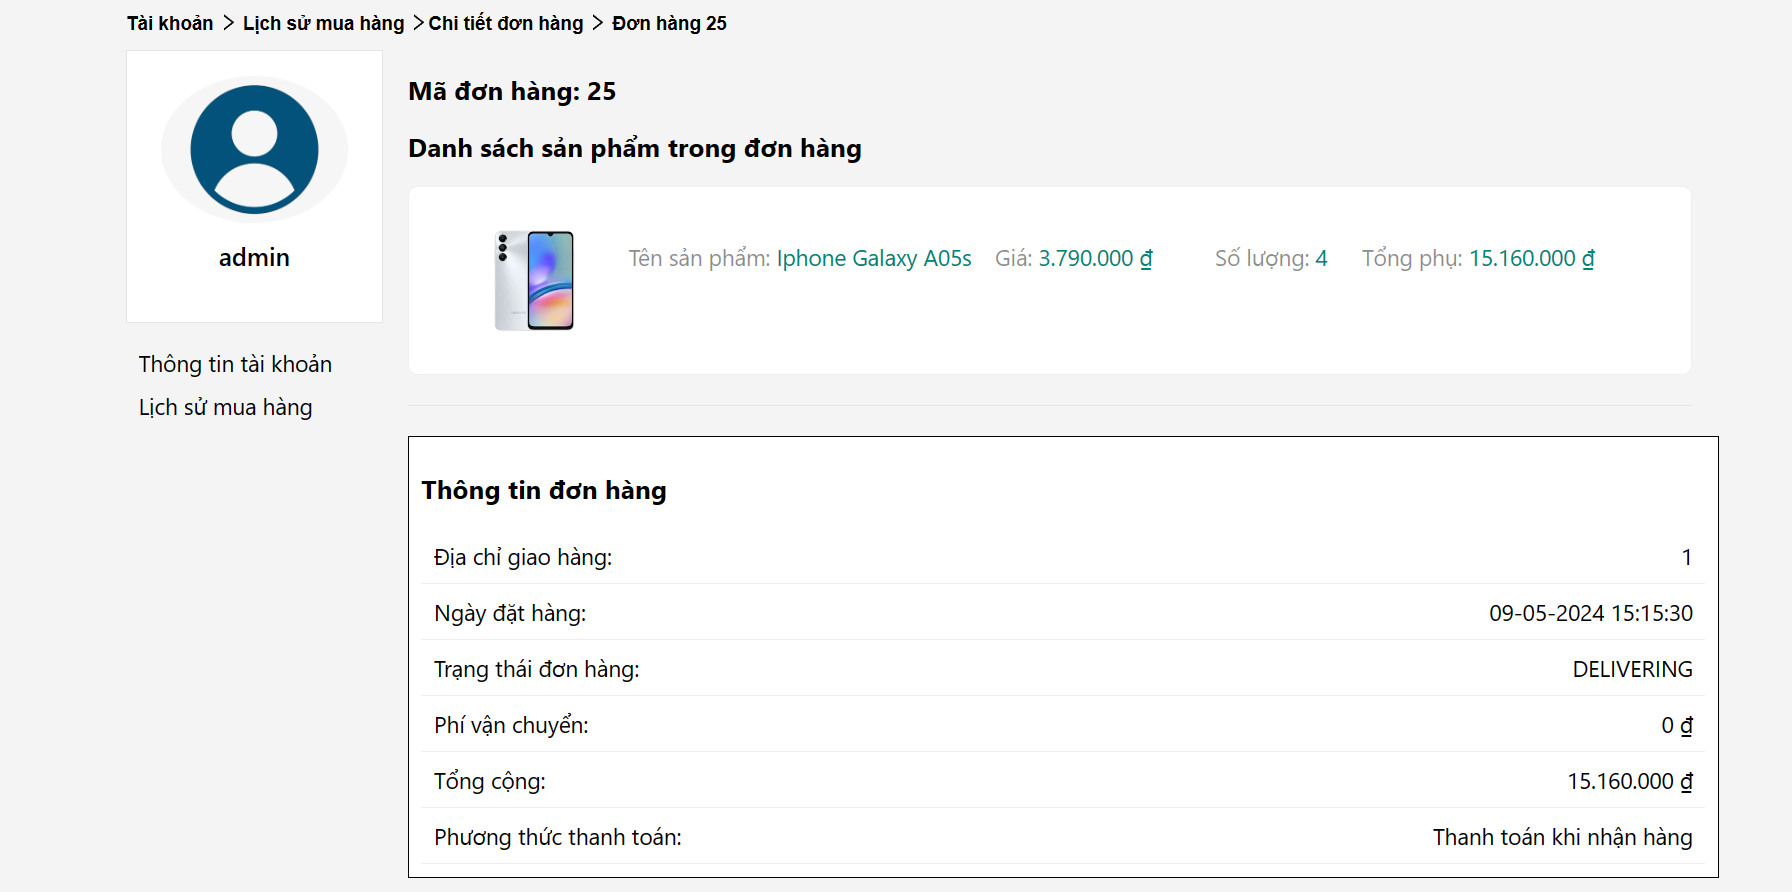
\includegraphics[scale=0.4]{images/hieu/chap-5/ordered-detail.png}
    \vspace*{3mm}
    \caption{Giao diện trang chi tiết đơn hàng}
    \end{center}
\end{figure}
\subsection{Trang quản lý tài khoản}
\begin{itemize}
    \item Hiển thị thông tin người dùng như: tên đầy đủ, email, số điện thoại.
    \item Thay đổi thông tin nếu muốn, nhấn lưu thay đổi để cập nhật lên hệ thống, tương tự với đổi mật khẩu.
\end{itemize}

\begin{figure}[H]
    \begin{center}
    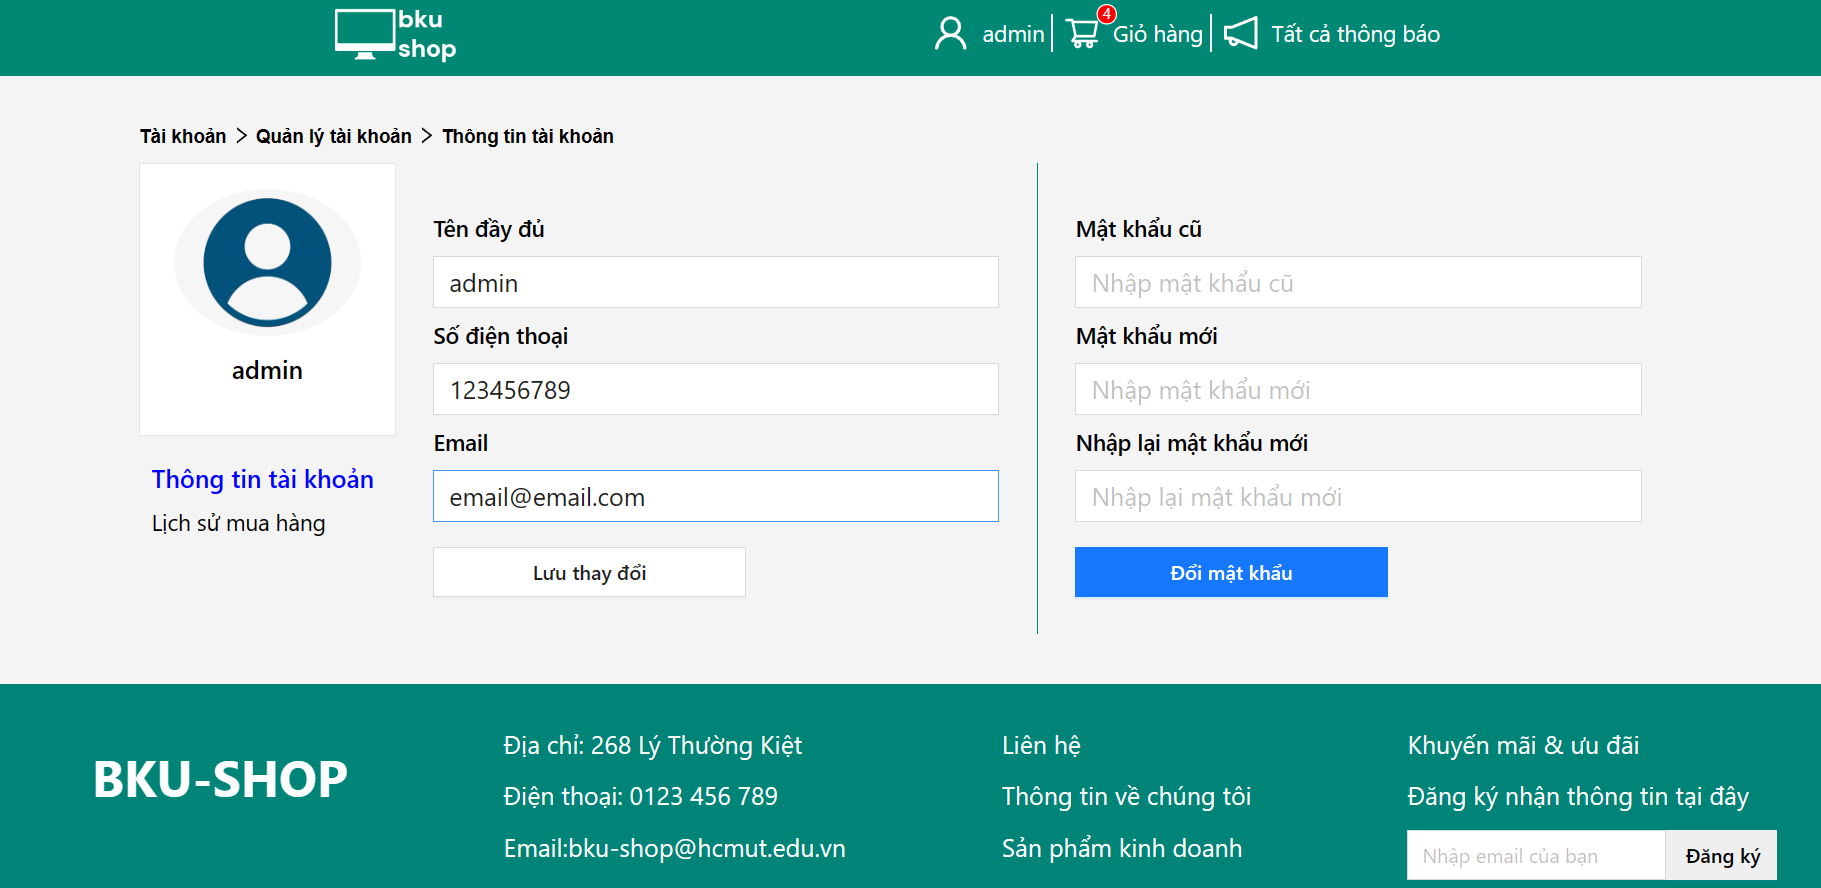
\includegraphics[scale=0.4]{images/hieu/chap-5/account.png}
    \vspace*{3mm}
    \caption{Giao diện trang quản lý tài khoản}
    \end{center}
\end{figure}
\subsection{Trang quản lý thông báo}
\begin{itemize}
    \item Hiển thị danh sách các thông báo mà hệ thống đã gửi cho người dùng.
    \item Hiển thị tất cả thông báo.
    \item Hiển thị riêng các thông báo chưa đọc.
    \item Thông tin chi tiết thông báo như: nội dung, thời gian.
    \item Nhấn từng thông báo để xem chi tiết.
    \item Cập nhật tất cả thông báo thành đã đọc nếu muốn.
\end{itemize}

\begin{figure}[H]
    \begin{center}
    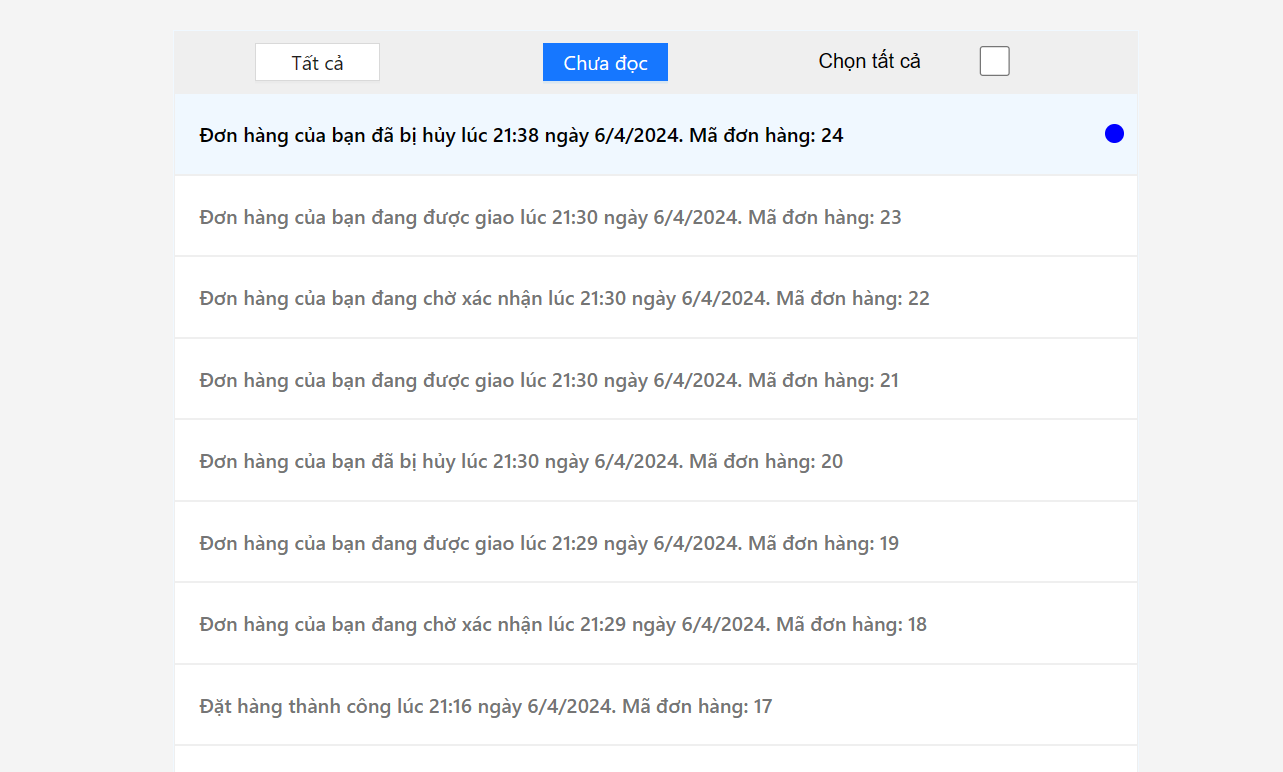
\includegraphics[scale=0.5]{images/hieu/chap-5/noti.png}
    \vspace*{3mm}
    \caption{Giao diện trang quản lý tất cả thông báo}
    \end{center}
\end{figure}
\begin{figure}[H]
    \begin{center}
    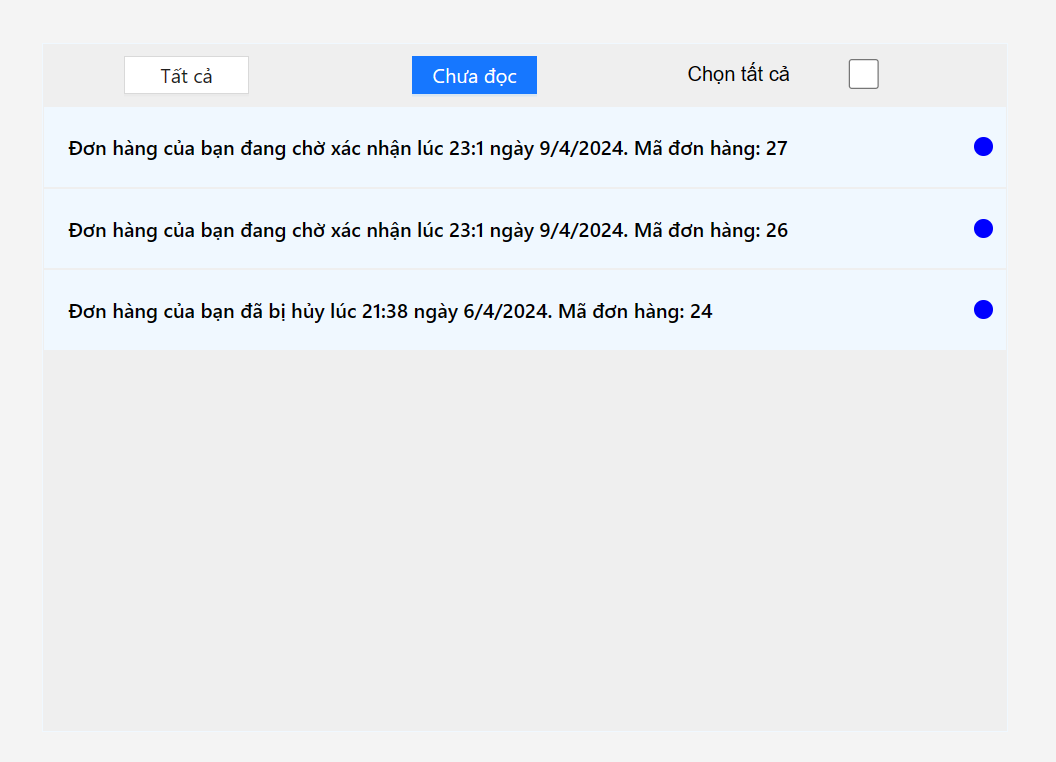
\includegraphics[scale=0.5]{images/hieu/chap-5/noti-notread.png}
    \vspace*{3mm}
    \caption{Giao diện trang quản lý thông báo người dùng chưa đọc }
    \end{center}
\end{figure}
\subsection{Giao diện popup thông báo mới}
\noindent Hiển thị danh sách các thông báo mới
\begin{figure}[H]
    \begin{center}
    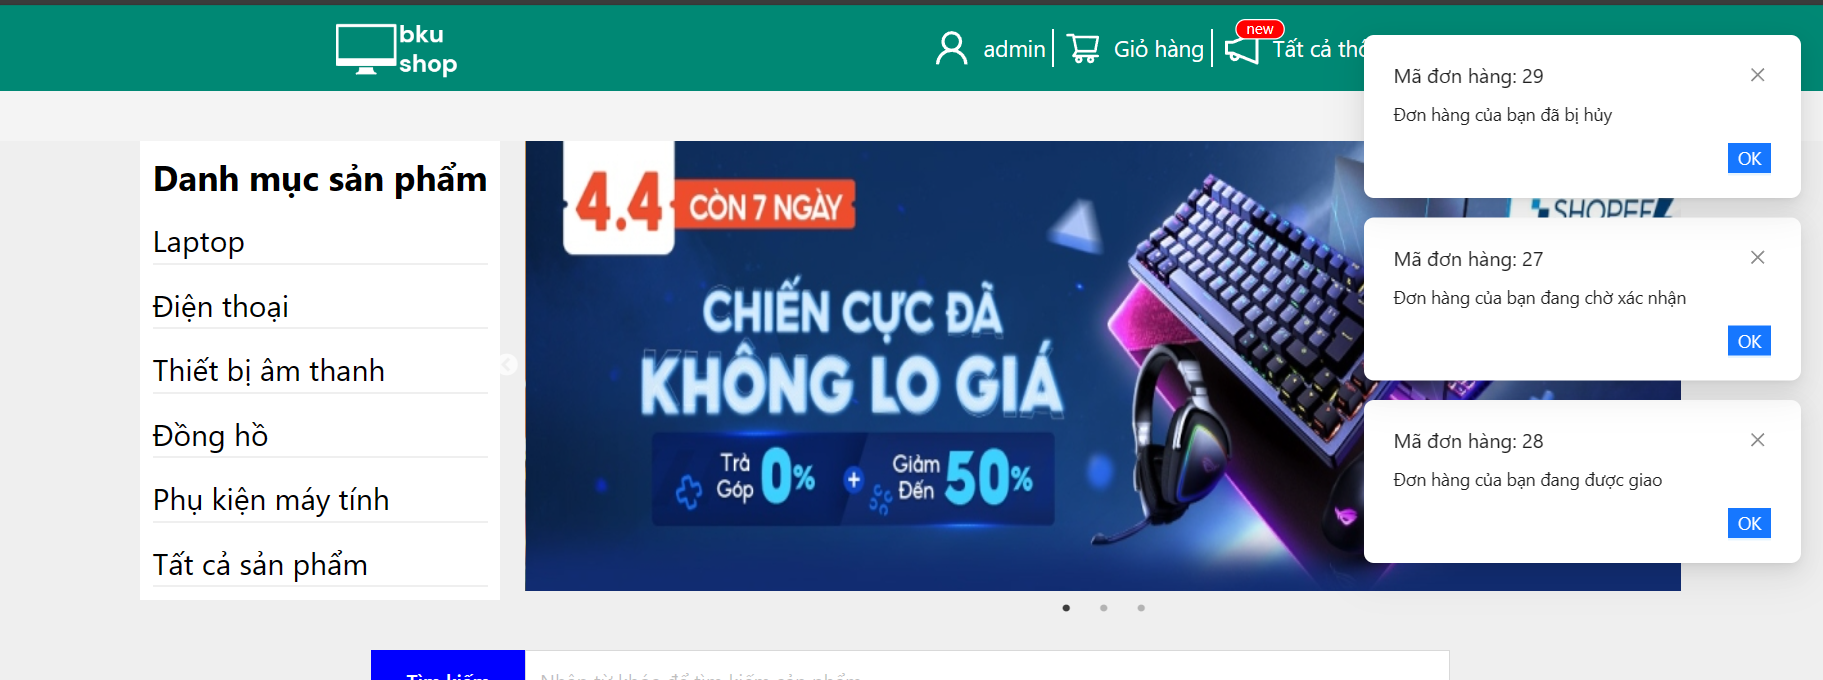
\includegraphics[scale=0.35]{images/hieu/chap-5/popup.png}
    \vspace*{3mm}
    \caption{Giao diện popup thông báo mới}
    \end{center}
\end{figure}